\chapter{Overview of techniques}
This chapter introduces the techniques used to simulate destructible environments. First, we will talk about the development of the destructible environment in several games and game engines, and then about general approaches to this problem.

We will repeatedly categorize the content of the game world in following way: We will use the word object to refer to any kind of building, crate, door, tree or other item that occurs in the game environment, but excluding terrain, distant environment like skyboxes, and any in-game characters.

%mozna by bylo fajn vedet proc zduraznujes ze to sou objekty a proc to je rozdilny od "normalni" definice objektu "cokoliv co jde uchopit dostatecne velkou rukou"

\section{Implementations in mainstream gaming} % tenhle nadpis je tezkej vymyslet dobre no :]

%Je fajn uvyst nasledujici seznam --- Tady ukazeme par metod ktery moh videt hrac ve hrach za poslednich 20 let a hodne her je pouziva docela silne.

\para{Object replacement or removal} was the first method used to simulate the destructible environment in a computer game, mostly because it is straightforward and undemanding. Despite its simplicity, it can still produce a very desirable result. In fact, it is still most widely used approach to the destructible environment in computer games.

%tady chybi definice proc to je object replacement/removal
%otazka: Jak poznam z nejaky hry ze to je object replacement/removal?

The first 2D games featuring destructible environment are arcade games like the \emph{Space Invaders (1978)}~\footnote{https://en.wikipedia.org/wiki/Space\_Invaders} where the environment is represented by cells in a grid. After taking damage, the texture of the cell is replaced by another one and the finally completely removed. The next\todo{in what ordering? isn't it just similar?} environment destruction technique in 2D games came with games like \emph{Scorched Earth (1991)}~\footnote{https://en.wikipedia.org/wiki/Scorched\_Earth\_(video\_game)} and \emph{Worms (1995)}~\footnote{https://www.team17.com/games/worms-original}. Collision and removal of terrain in those games is based on individual pixels which create a more realistic visual effect.

%problem s kategorizaci: pred chvilkou se mluvi o destrukci celych prostredi, tady najednou jen o destrukci objektu. Bylo by fajn rovnou zminit ze ve 3d hrach se niceni prostredi moc nepouziva a likvidujou se jen ty objekty.
The most common implementation of destructible objects in 3D games has not changed much over the years. Every object that the player can modify has a set of more damaged models prepared. Based on how much damage is applied, the models are swapped and eventually completely removed, as seen in \cref{fig:doors}. It is usually accompanied by animations, debris and dust generation to make the process look realistic. The downfall of this method is the necessity to replace the whole in-game object. There has to be a significant number of objects pre-made for different scenarios to make the game look realistic and it has little flexibility to react to specific player actions. As an example, in the \emph{Source} engine, the hole in the door (\cref{fig:doors}) is always in the same place, regardless of the point of impact.

%Co by melo bejt doplneny:
%Magic carpet (1994?) a Starfighter3000 (1991?) byl 3D a de tam likvidovat teren. (potencialni rozpor s predchozim odstavcem)
%Duke Nukem 3D: Predpripraveny "popraskany steny" ktery jdou prostrelit bazukou.

\begin{figure} %na parametry {figure} je dobry se uplne vykaslat, tex ty mista vetsinou zvoli nejlip, aby nerusily tok textu. Doporucuju [t] kdyz automaticka volba mista fakt hodne selze, [p] kdyz mas hodne obrazku a je dobry je odhazet na jednu stranku (viz niz), a [b] v krizi. Pokud neco potrebujes fakt primo do textu, tak to vubec nedavej do {figure} environmentu
\centering
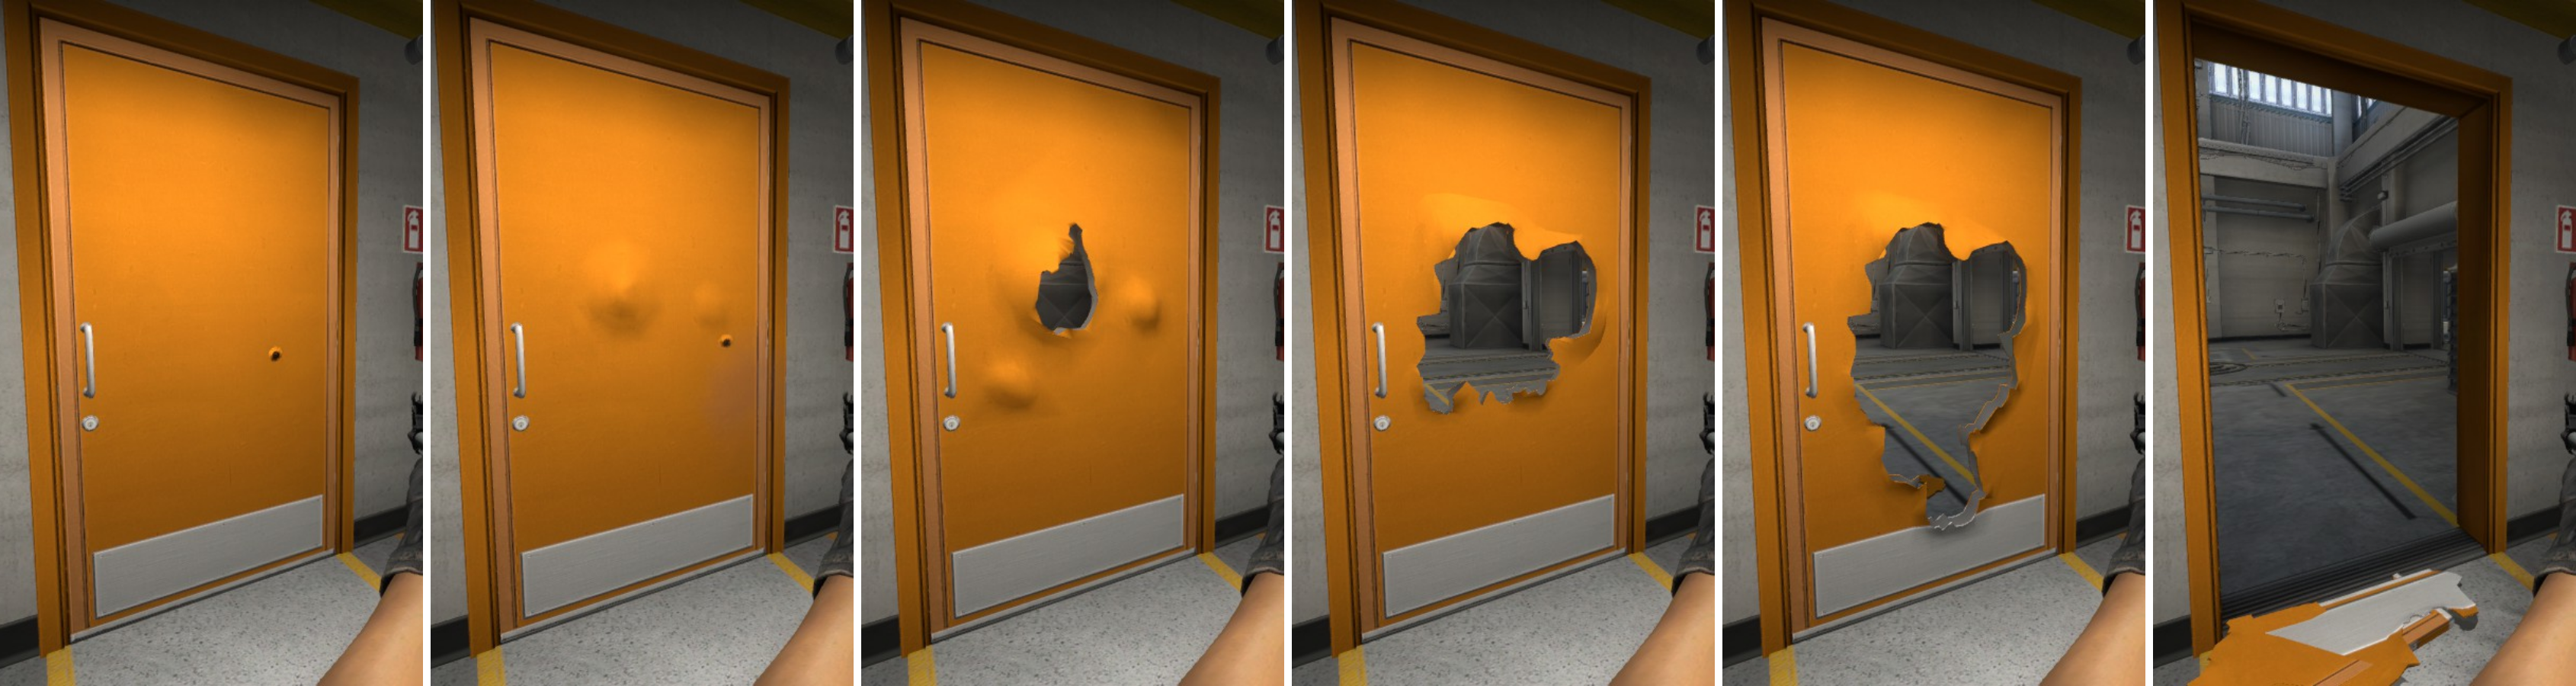
\includegraphics[width=\textwidth]{img/doors}
% k obrazkum je vzdycky potreba napsat neco co si z nich ma odnyst nahodnej kolemjdouci kterej kouka jen na obrazky. Napr.:
\caption{\emph{Source} engine swaps door models. Image taken from ???. Successively damaging any doors in the game will always produce this sequence of models, regardless of the exact point where the damage is applied.}
\label{fig:doors}
\end{figure}

%tady zduraznit ze to je prvni 3d hra ktera s tim vysla fakt na povrch
\para{\emph{Geo-Mod}} (\emph{Geometry Modification Technology}\cite{geomod}) is an engine developed for the \emph{Red Faction (2001)}\footnote{http://redfaction.wikia.com/wiki/Red\_Faction} video game. It allows players to modify and make holes in the terrain using the solution of creating objects representing an empty space. The difference of meshes is calculated in real time to represent the terrain with a hole. Even though the engine does not work well with the buildings and other objects, it represents one of the first significant attempts to create the fully destructible 3D environment in real time constraints.

\para{\emph{Geo-Mod 2}}~\cite{geomod}\footnote{Geo-Mod 2.0 presentation video https://www.youtube.com/watch?v=lICurOVsNv0} does not feature destructible terrain, instead, it uses physics simulation on specially prepared objects. A set of smaller objects is used as a ragdoll for the stress-based simulation model. The complexity of simulation limits the engine in the scale of the game world and mutual proximity of destructible objects.


\para{\emph{Frostbite}}~\footnote{http://www.frostbite.com/about/frostbite-3} engine and mainly it's component \emph{Destruction}~\cite{destruction} is currently used in the most titles featuring destructible environment. It supports the dynamic micro-destruction on the surface and the large scale predetermined destruction on whole buildings. For the large-scale destruction, the buildings are created from smaller parts linked together. Each part can disappear on its own, and when there is not enough left, the whole building collapses. It does not use internal body stress or any physics while doing this simulation. \emph{Frostbite} is a proprietary engine and there is no public information on the implementation of micro-destruction.

\section{Methods and algorithms}

Here we give a short overview of several more rigorous methods commonly used in current games.

\subsection{Soft body deformation}

% Je textove-strukturni chyba mit pod nadpisem hned seznam bez vysvetleni co ten seznam dela.

\para{Finite Element Method} (FEM) is an approach to simulate the behaviour of complex objects and systems\todo{jak moc komplexni musej bejt aby na ne byla potreba FEM?}. It uses a large number of finite volumes (cells), interconnected or not, to simulate the reaction of material to inner and outside forces. Each cell calculates its physics states like stress or temperature and propagates the results to neighbouring cells. This model allows for simulation of fluid dynamics, brittle fractures~\cite{brittlefracture}, ductility~\cite{ductilefracture}, elasticity, heat transfer and other physical properties. It is beneficial in engineering, modelling and rendering scenes for computer generated images but FEM requires a lot of computational resources and therefore until recently it was not possible to implement it in real-time environment of a computer game. Now with better hardware and optimised algorithms especially developed for real-time animation, like the one O'Brien~\cite{femingames} describes this method is making its way into modern games.

\para{Material Point method} (MPM) is used to simulate the behaviour of continuum materials. MPM is a meshfree and Arbitrary Lagrangian–Eulerian numerical method \cite{ALE}. The Lagrangian element, or a material point, is the primary representation possessing position, velocity and deformation gradient. A simplified overview of algorithm steps follows, for more details see the thesis of \citet{jiang2015material}.

\begin{enumerate}
    \item Grid data are reinitialized to default values.
    \item Weights and weight gradients are computed on every particle.
    \item Mass and momentum are transferred from the particles to the grid.
    \item The explicit forces on nodes are computed
    \item The explicit nodal velocity update is performed
    \item Grid based collision is performed on vertices.
    \item Particles are updated from grid velocities.
\end{enumerate}
The steps are illustrated in \cref{fig:mpm}.

MPM is useful for both fluid and soft body dynamics. It can simulate deformation, fractures, heat transfer, melting and other changes of material properties.

\begin{figure}
\centering
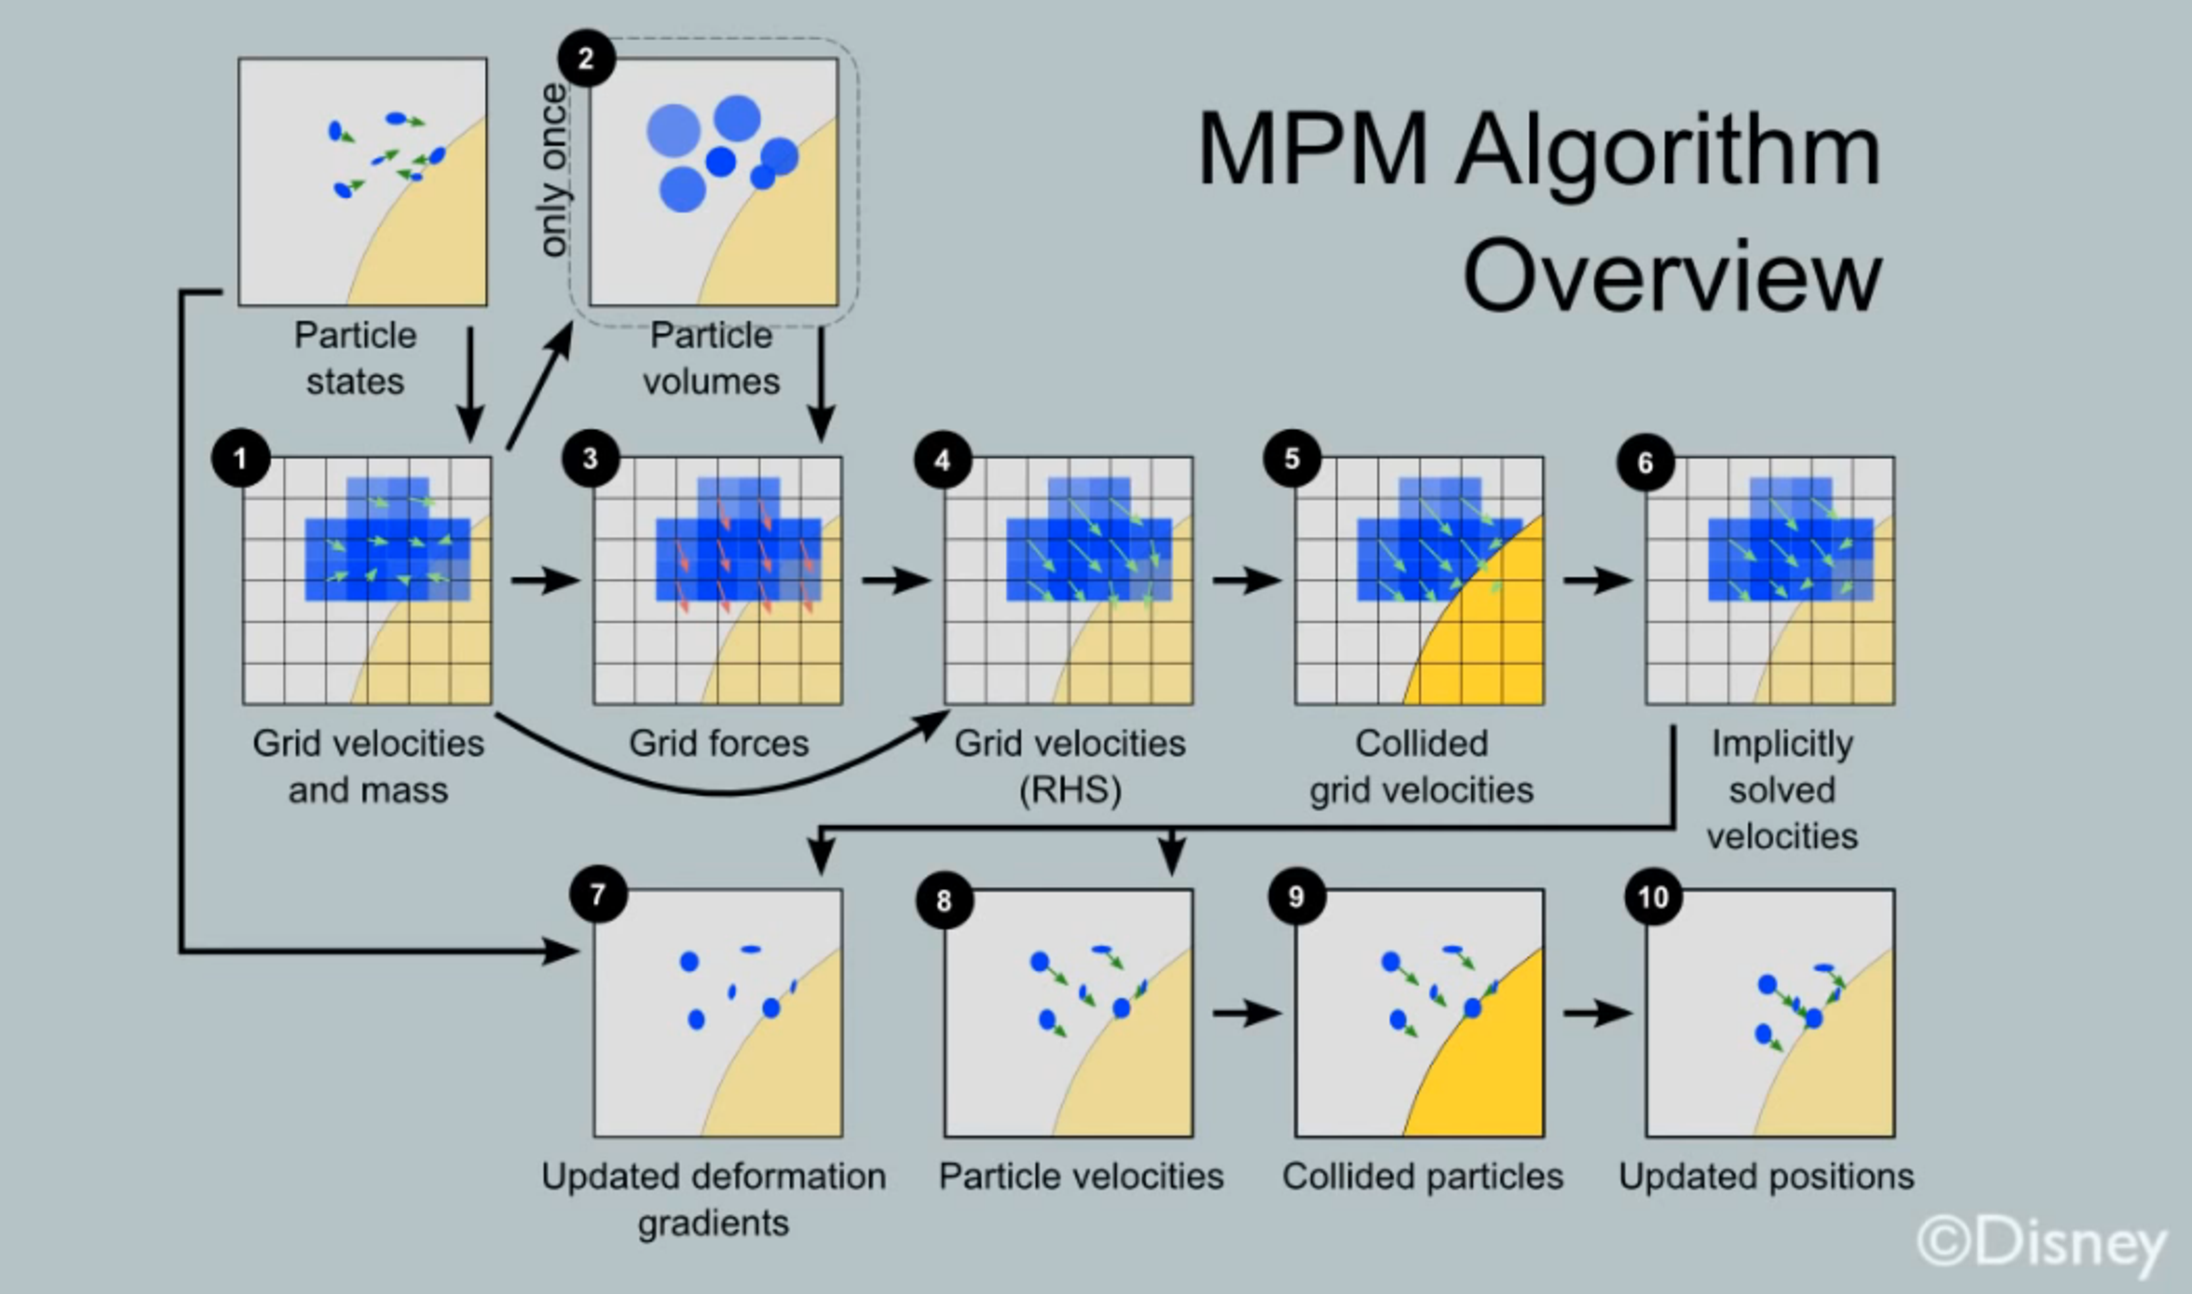
\includegraphics[width=\textwidth]{img/MPM}
\caption{MPM algorithm overview. The top and the bottom rows operate in particle domain (Lagrangian) while the middle depicts grid-based (Eulerian) operations \cite{disney}.
}
\label{fig:mpm}
\end{figure}

\subsection{Rigid body decomposition}

%Proc se kapitola jmenuje R.b.d. a jak to souvisi s tim ze najednou tady je Voronoi tesselation?
%Treba:
Decomposition of rigid bodies is used to make the object appear broken, or introduce damage into a 3D polyhedral solid. The most common method used today is Voronoi tesselation.
% (asi to prepis. :D )
There are also other solutions for decomposition, \eg slicing by planes or convex decomposition, but Voronoi cells are considered to look better and more natural than other methods. 

\para{Voronoi tessellation} is a method of decomposing an object into a smaller parts, as shown on \cref{fig:voro}. It is also applicable for \eg terrain generation\todo{referenci na definici "terrain generation"}, but we will focus on object decomposition. The tessellation can be done in following three steps, assuming the input is a closed triangular mesh with non-empty volume:
\begin{description}
    \item[Delaunay tetrahedral decomposition] Given points $P$ in general position (the vertices of input mesh and a set of points inside its volume), tetrahedral mesh $DT(P)$ can be generated satisfying the following condition: no point in $P$ is inside the circumscribed sphere of any tetrahedra in $DT(P)$.
    \item[Creating Voronoi diagram] For a Delaunay tetrahedral decomposition, its dual graph (with vertices in the centre of tetrahedrons circumscribed sphere) is a Voronoi diagram.
    \item[Clipping the Voronoi diagram] Boundary cells of the Voronoi diagram are infinite (see \cref{fig:DT}) and need to be clipped by the original input triangular mesh. The efficient algorithm~\cite{yan2010efficient} for this task finds the intersection of the boundary Voronoi cell with the triangular mesh and continues with neighbourhood propagation to determine all intersections. 
\end{description}

\begin{figure}
	\centering
	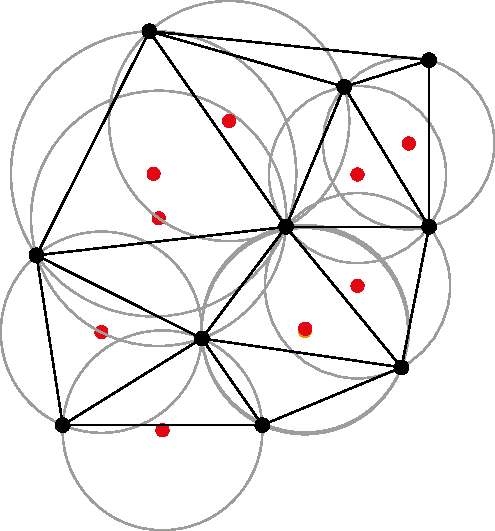
\includegraphics[width=0.4\textwidth]{img/delaunay}
	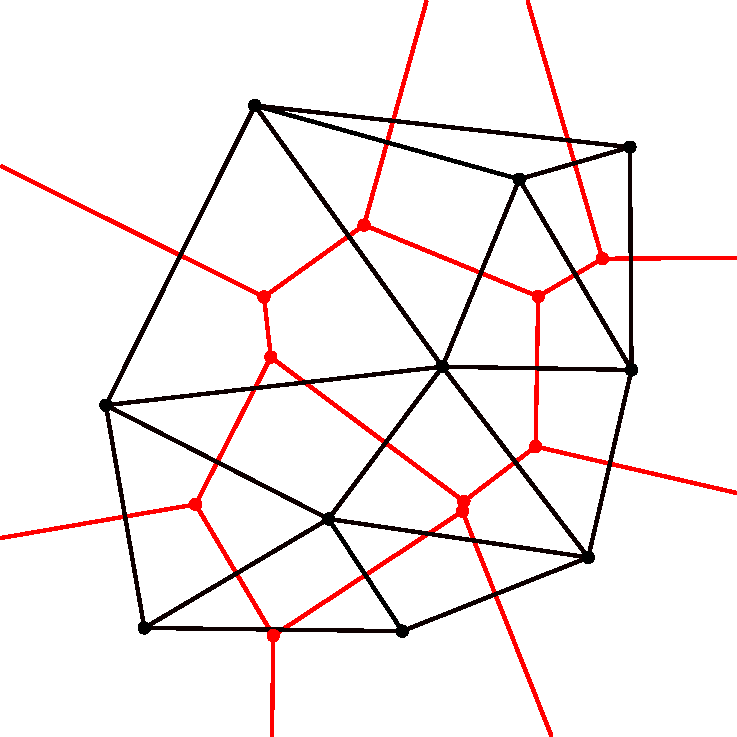
\includegraphics[width=0.4\textwidth]{img/voronoi}
	\caption{Transformation of 2D Delaunay triangulation to Voronoi diagram. Source: \url{https://en.wikipedia.org/wiki/Delaunay\_triangulation}}
	\label{fig:DT}
\end{figure}
\begin{figure}
        \centering
        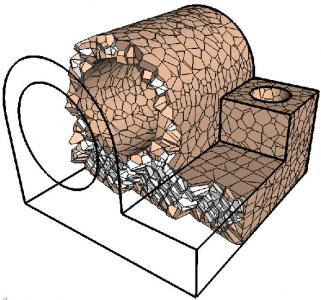
\includegraphics[width=0.4\textwidth]{img/clipped}
        \caption{The result of Voronoi tessellation \cite{yan2010efficient}}
        \label{fig:voro}
\end{figure}

